\chapter{Theory}
\label{chap:theory}

\section{Heat Transfer}
\label{chap:heat_transfer}
Heat transfer is the phenomenon of thermal energy being transported as a result of spatial temperature differences \cite{Bergman_2011}. In thermodynamics, heat can be transferred by three modes, conduction, convection and radiation. While it is important to describe how energy can be transferred, energy can also be stored in materials. Just by heating materials, the heat pumped in can be stored and transferred back later either by latent heat storage, or sensible heat storage. 

\subsection*{Conduction}
Conduction is the energy transfer from highly energetic particles to low energetic particles. The energy is transferred by the interactions between the particles. Essentially, when a high-energy particle collides with a low-energy particle, some of that energy is transferred to the lower-energy particle. However, the key difference separating it from convection, is there is no bulk motion \cite{Bergman_2011}. In gasses, conduction occurs when particles, which move freely but are spaced far apart, collide. In liquids, the same phenomenon occurs, but the particles are much closer together so collisions are more frequent. And lastly, in solids, it relates to the oscillations of the lattice structure and the movement of free-flowing electrons. Figure \ref{fig:conductivity_of_materials} shows the thermal conductivities of various materials.
\begin{figure}[ht]
	\centering
	\includegraphics[width=0.75\linewidth]{figures/chapter_2/Conductivity.png}
	\caption{Range of thermal conductivities in different materials \cite{Bergman_2011}}
	\label{fig:conductivity_of_materials}
\end{figure}

Conduction can be described by Fourier's law, shown in equation \ref{eq:fouriers_law}, where $q$ represents a given heat flux, $k$ is the thermal conductivity of the material and $\nabla T$ is the temperature gradient. 
\begin{equation}
	q = k \nabla T
	\label{eq:fouriers_law}
\end{equation}

Fourier's law of conduction describes a system that has reached a steady state. To describe a transient system, the heat equation, shown below in equation \ref{eq:heat_equation}, can be used. This equation can describe the temperature evolution over time $\partial_tT$, given the density $\rho$, specific heat capacity $c_p$, thermal conductivity $k$ as well as the heat generation $q$ are known \cite{Bergman_2011}.
\begin{equation}
	\rho c_p \partial_tT=\nabla\cdot\nabla (kT) + q
	\label{eq:heat_equation}
\end{equation}

When the thermal conductivity remains constant or varies very little over the temperature range that is being investigated, the heat equation can be rewritten in the form shown in equation \ref{eq:heat_eq_simple} where $\alpha=k/\rho c_p$ is a diffusion coefficient \cite{Bergman_2011}. The diffusion coefficient relates the ability of a material to conduct heat relative to its ability to store heat \cite{Bergman_2011}. For example, materials with a small diffusion coefficient can't conduct the heat away so they need to store it until they reach a new equilibrium.
\begin{equation}
	\frac{1}{\alpha}\partial_tT=\nabla^2T + \frac{q}{k}
	\label{eq:heat_eq_simple}
\end{equation}

The heat flux in the heat equation can come from multiple sources. For example, heat can be generated internally by chemical reactions or by electrical heating. However, the other heat transfer modes, convection and radiation, can add or subtract from the heat flux. 

\subsection*{Convection}
Convection is comprised of both conduction and heat transfer resulting from bulk fluid motion \cite{Bergman_2011}. Because the thermal conductivity of low, it is the bulk fluid motion that dominates this form of heat transfer. Two forms of convection exist, either forced convection or natural convection. In both cases, equation \ref{eq:heat_convection} can be used to predict the temperature gradient between an interface, given some convection coefficient $h$ \cite{Bergman_2011}, which is often determined empirically. Note that $q$ is a heat flux.
\begin{equation}
	q = h\Delta T
	\label{eq:heat_convection}
\end{equation}

In forced convection, the fluid is driven to flow by an external device such as a fan. Many empirical relations exist which can be used to determine the convection coefficient. In the case of forced convection, they usually revolved around determining the Nusselt number $\textit{Nu}_x$ which is commonly a function of the Reynold's number $\textit{Re}$ and the Prandtl number $\textit{Pr}$. Once the Nusselt number is known, the convection coefficient can be determined from equation \ref{eq:nusselt_convection}.
\begin{equation}
	h = \frac{k\textit{Nu}_x}{x}
	\label{eq:nusselt_convection}
\end{equation}

In natural or free convection, fluid motion occurs as a result of slight density changes in the fluid \cite{Bergman_2011}. The convection coefficient in this case is usually much lower, as heat is advected much slower. The Nusselt number in free convection usually depends on the Grashof number $\textit{Gr}_x$.
\begin{equation}
	\textit{Gr}_x = \frac{g\beta\Delta T x^3}{\nu^2}
	\label{eq:grashof_number}
\end{equation}

In reality, to capture the fluid motion and temperature distribution throughout a domain, the Navier-Stokes equations are needed. To solve these, numerical methods such as the finite-element method, or finite-volume method are used. This is computationally expensive, which is why a great deal of work has gone into determining convection coefficients for simple problems.

\subsection*{Radiation}
Radiation differs from the previous two modes of heat transfer in that it does not require a transfer medium. In radiation, heat is transferred by photons which are emitted from any material of non-zero temperature \cite{Bergman_2011}. Energy is emitted according to equation \ref{eq:radiation_emission}, where $\epsilon$ is the material emissivity which describes how close to an ideal radiator the material is, and $\sigma=5.67\times 10^{-8}$ is the Boltzmann constant \cite{Bergman_2011}. 
\begin{equation}
	E = \epsilon\sigma T_s^4
	\label{eq:radiation_emission}
\end{equation}

Because all materials emit radiation, some of the energy emitted by the surface will return. Therefore, heat transfer by radiation is described as a net transfer rate, meaning the temperature differences between mediums are still important. This is shown in equation \ref{eq:radiation_transfer} where $T_s$ is the temperature of the surface of the material, $T_{sur}$ is the temperature of the surroundings, and $q$ is a heat flux.
\begin{equation}
	q = \epsilon\sigma(T_s^4 - T_{sur}^4)
	\label{eq:radiation_transfer}
\end{equation}


\section{The Stefan Problem}
\label{chap:stefan_problem}
The Stefan problem is a particular kind of heat transfer problem that involves the melting or freezing of a material, giving rise to the movement of an interface within the domain. Josef Stefan developed the theory in the years surrounding 1890 and compared his findings to data that had been obtained during polar expeditions \cite{1889aSTEFAN}\cite{1889bSTEFAN}\cite{1889cSTEFAN}\cite{1891STEFAN}. The classical Stefan problem assumes the fluid domain to be at rest. 
\begin{figure}[ht]
	\centering
	\includegraphics[width=0.7\linewidth]{figures/chapter_2/StefanProblem.png}
	\caption{Illustration of the Stefan problem}
	\label{fig:stefan_problem}
\end{figure}

For simplicity, this analysis, based on notes from \cite{Kowalski_2022}, will consider an initial domain of ice that is all at the melting temperature $T(x,0) = T_m$. This is often referred to as the one-phase Stefan problem as the temperature distribution is only solved in the fluid domain. If a heat source is applied to the left side of the domain, the melt front position $X(t)$ will begin moving through the domain. In the fluid domain, the heat equation can be solved in the domain $0\leq x\leq X(t)$. Equation \ref{eq:interface_temperature} shows the interface boundary condition where $X^-(t)$ denotes the fluid side of the boundary, and $X^+(t)$ denotes the solid side of the boundary.
\begin{equation}
	T(X^-(t),t) = T(X^+(t),t) = T_m
	\label{eq:interface_temperature}
\end{equation}

To close the equation, the position of the interface needs to be determined. One final boundary condition, called the Stefan condition is required. As shown in equation \ref{eq:stefan_condition} it represents a local energy balance at the interface to account for the jump caused by the latent heat $L$. In the one-phase problem, the temperature gradient in the solid is zero, leaving only the liquid contribution as shown in equation \ref{eq:stefan_condition_onephase}.
\begin{subequations}
	\begin{equation}
		\rho_sL\partial_tX(t)=k_s\partial_xT(X^+(t),t) - k_l\partial_xT(X^-(t),t)
		\label{eq:stefan_condition}
	\end{equation}
	\begin{equation}
		\rho_sL\partial_tX(t)=- k_l\partial_xT(X^-(t),t)
		\label{eq:stefan_condition_onephase}
	\end{equation}
\end{subequations}

Now that the system is closed, a solution can be found by introducing a similarity variable $\zeta=x/\sqrt{t}$. After solving and back-substitution, the final temperature profile can be determined as shown in equation \ref{eq:temperature_stefan}, where $T_l$ is the temperature on the left boundary, and the error function $\text{erf}(x):=\frac{2}{\sqrt{x}}\int_0^x e^{-y^2}dy$.
\begin{equation}
	T(x,t) = T_l - (T_l-T_m)\frac{\text{erf}(\frac{x}{2\sqrt{\alpha t}})}{\text{erf}(\frac{X(t)}{2\sqrt{\alpha t}})}
	\label{eq:temperature_stefan}
\end{equation}

The final thing to determine is the position of the interface. This can be done by making use of the Ansatz function $X(t)=2\sqrt{\alpha}\lambda\sqrt{t}$. This function introduces the unknown variable $\lambda$ which can be found by substituting the Ansatz function into the Stefan condition, which results in equation \ref{eq:stefan_lambda}. 
\begin{subequations}
	\begin{equation}
		\lambda\sqrt{\pi}=\frac{c_p(T_l-T_m)}{L}\frac{1}{\text{erf}(\lambda)e^{\lambda^2}}=\text{Ste}^{-1} \frac{1}{\text{erf}(\lambda)e^{\lambda^2}}
		\label{eq:stefan_lambda}
	\end{equation}
	\begin{equation}
		g(\lambda)=\text{Ste}^{-1}-\sqrt{\pi}\lambda e^{\lambda^2}\text{erf}(\lambda) = 0
		\label{eq:solve_for_lambda_stefan}
	\end{equation}
\end{subequations}

Equation \ref{eq:stefan_lambda} cannot be directly solved for $\lambda$, so the equation is reformulated to be solved for a root instead as shown in equation \ref{eq:solve_for_lambda_stefan}. This equation can be solved using a root finder. An example of how the front develops is shown in figure \ref{fig:melt_front_movement}. In this example, the material properties of water were used.
\begin{figure}[ht]
	\centering
	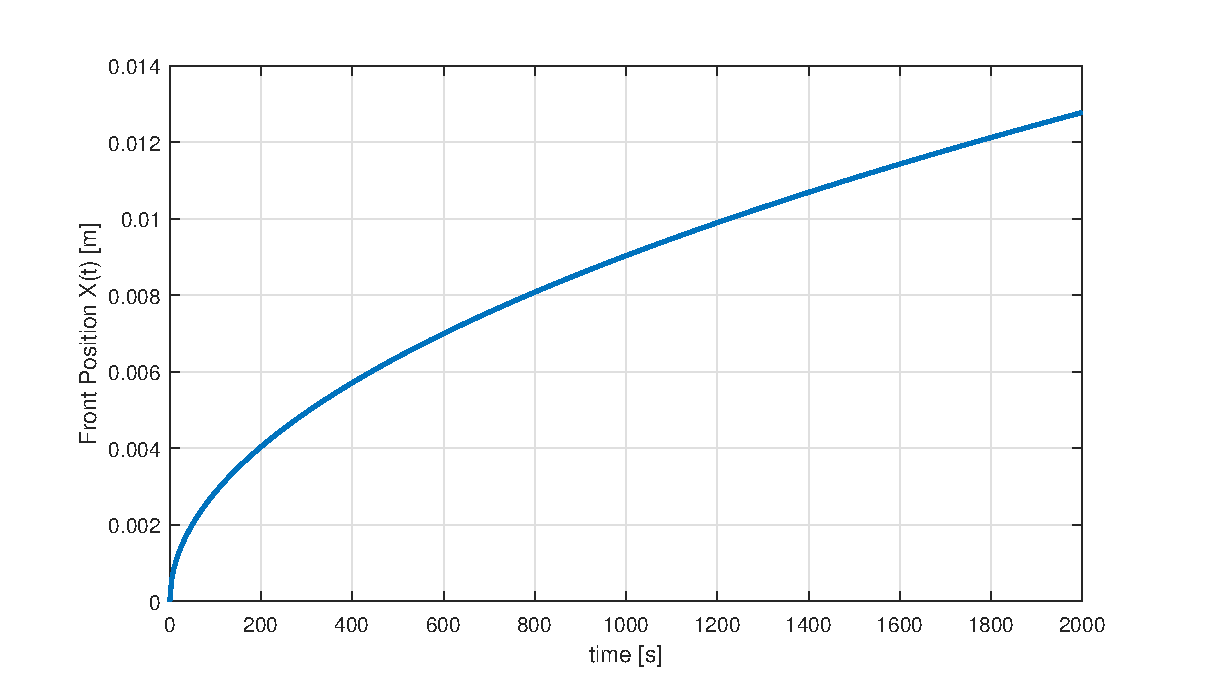
\includegraphics[width=0.9\linewidth]{figures/chapter_2/StefanFront.eps}
	\caption{Stefan melting front development over time}
	\label{fig:melt_front_movement}
\end{figure}


\section{Structural Mechanics}
\label{chap:solid_mechanics}
The main idea of structural mechanics is that a material deforms under a load. This gives rise to shear and normal stress in the material. It is usually enough to consider materials to behave linearly. This gives rise to the classical Hooke's law, which can be generalized for a multidimensional object. Continuum mechanics also needs to be considered for the derivation, but for simplicity, it is not discussed in this thesis.

\begin{figure}[ht]
	\centering
	\includegraphics[width=0.8\linewidth]{figures/chapter_2/StretchedBar.png}
	\caption{One-dimentional Hooke's law illustration}
	\label{fig:stretched_bar}
\end{figure}
First considering the one-dimensional case as illustrated in figure \ref{fig:stretched_bar}. A simple bar of length $L$ with cross-sectional area $S$ is subjected to a load $P$. Under this load, the bar stretches in the longitudinal direction by $\Delta L$ and contracts by $\Delta S$ in the perpendicular direction. Classical Hooke's law states that this stretching can be determined, as shown in equation \ref{eq:hookes_law} \cite{Lubliner_Papadopoulos_2014}. The contraction can also be computed from equation \ref{eq:hookes_law_contraction}, where $\nu$ is Poisson's ratio.
\begin{subequations}
	\begin{alignat}{2}
		\frac{\Delta L}{L} &= \frac{1}{E}\frac{P}{S} 
		\label{eq:hookes_law} \\
		\frac{\Delta S}{S} &= \nu\frac{\Delta L}{L}=\nu\frac{1}{E}\frac{P}{S} 
		\label{eq:hookes_law_contraction}
	\end{alignat}
\end{subequations}

Equation \ref{eq:hookes_law} is most commonly written as $\sigma=E\epsilon$ where $\sigma=P/S $ and $\epsilon=\Delta L/L$. In solid mechanics, the strain is usually $\mathcal{O}(10^{-3})$ while Young's modulus $E$ is usually $\mathcal{O}(10^6)$. Assuming the rod returns to its original form after the load is released, Hooke's law can be generalized and derived through continuum mechanics, and the linear, elastic material model can be determined. Equation \ref{eq:linear_elastic_material} shows this.
\begin{equation}
	\sigma=\lambda\text{tr}(D)\mathbf I + 2\mu D
	\label{eq:linear_elastic_material}
\end{equation}

The linear elastic model of materials introduces so-called Lam\'{e} parameters $\lambda$ and $\mu$ which can be calculated for each material, given its material properties are known, as shown in the equations \ref{eq:lame_equations}. It also introduces $D$, the small-strain tensor defined in equation \ref{eq:small_strain_tensor}.
\begin{subequations}
	\begin{equation}
		D =
		\begin{bmatrix}
			\epsilon_{xx} & \epsilon_{xy}  & \epsilon_{xz} \\
			\epsilon_{yx} & \epsilon_{yy}  & \epsilon_{xz} \\
			\epsilon_{zx} & \epsilon_{zy}  & \epsilon_{xz}
		\end{bmatrix}
		\label{eq:small_strain_tensor}
	\end{equation}
	\begin{equation}
		\lambda = \frac{\nu E}{(1+\nu)(1-2\nu)} \qquad \mu = \frac{E}{2(1+\nu)}
		\label{eq:lame_equations}
	\end{equation}
\end{subequations}

Considering a three-dimensional case, stress occurs in six ways. Three in the normal directions, and three in the shear planes. A compliance matrix can be found for the system $\epsilon=\mathbf{C}^{-1}\sigma$ can be determined for a general material as shown in equation \ref{eq:elasticity_matrix}, which includes the shear modulus $G_{ij}$ \cite{Lubliner_Papadopoulos_2014}.
\begin{equation}
	\mathbf{C}^{-1}=\begin{bmatrix}
		\frac{1}{E_x} & \frac{\nu_{xy}}{E_x} & -\frac{\nu_{xz}}{E_x} & 0 & 0 & 0 \\
		-\frac{\nu_{yx}}{E_y} & \frac{1}{E_y} & -\frac{\nu_{yz}}{E_y} & 0 & 0 & 0 \\
		-\frac{\nu_{zx}}{E_z} & -\frac{\nu_{zy}}{E_z} & -\frac{1}{E_z} & 0 & 0 & 0 \\
		0 & 0 & 0 & \frac{1}{G_{yz}} & 0 & 0 \\
		0 & 0 & 0 & 0 & \frac{1}{G_{xz}} & 0 \\
		0 & 0 & 0 & 0 & 0 & \frac{1}{G_{xy}} \\
	\end{bmatrix}
	\label{eq:elasticity_matrix}
\end{equation}

Often, the materials are isotropic which gives the material uniform material properties in each direction. As in some cases, such as in 2D, the $z$ component of stress and strain are equal to or negligible. This simplifies the matrix as shown in \ref{eq:plane_stress} for plane stress
\begin{equation}
	\mathbf C^{-1} = \frac{1}{E}\begin{pmatrix}
		1 & -\nu & 0 \\
		-\nu & 1 & 0 \\
		0 & 0 & 2(1+\nu)
	\end{pmatrix}
	\label{eq:plane_stress}
\end{equation}
or to the equation shown in \ref{eq:plane_strain} for plane strain \cite{Lubliner_Papadopoulos_2014}.
\begin{equation}
	\mathbf C = \frac{E}{1+\nu} \begin{pmatrix}
		\frac{1-\nu}{1-2\nu} & \frac{\nu}{1-2\nu} & 0 \\
		\frac{\nu}{1-2\nu} & \frac{1-\nu}{1-2\nu} & 0 \\
		0 & 0 & \frac{1}{2}
	\end{pmatrix}
	\label{eq:plane_strain}
\end{equation}


\section{Methods for Optimization}
\label{chap:methods_for_optimization}
In the context of engineering, the goal of optimization is to maximize or minimize one or more properties, possibly with a set of constraints. Typical examples include maximizing the stiffness of a frame while keeping the design below a weight requirement, or minimizing the mass of a bridge while ensuring the maximum stress is below some critical limit. In optimization, a maximum is equivalent to a minimum \cite{Kochenderfer_Wheeler_2019}. This allows the same optimization methods to be used for any function.
\begin{equation}
	\begin{matrix}
		\max_x f(x) \\
		\text{is equivalent to} \\
		\min_x -f(x)
	\end{matrix}
\end{equation}

In optimization, a constraint limits the design space of possible solutions \cite{Kochenderfer_Wheeler_2019}. Figure \ref{fig:constraint_example} shows a function with a global and local minimum. The $\chi$ variable denotes the constraint limiting the design space, and $x^*$ is the optimum that fulfills the design criteria.
\begin{figure}[ht]
	\centering
	\includegraphics[width=0.6\linewidth]{figures/chapter_2/ContraintExample.png}
	\caption{Example of a constraint limiting the design space \cite{Kochenderfer_Wheeler_2019}}
	\label{fig:constraint_example}
\end{figure}

\subsection*{Constrained Optimization}
This section will consider the following system.
\begin{equation}
	\begin{split}
		\min_x \quad &f(\mathbf x) \\
		\text{subject to} \quad & h(\mathbf x) = \mathbf 0\\
		& g(\mathbf x) \leq \mathbf 0
	\end{split}
\end{equation}
As was briefly introduced, constrained optimization has a function that has had its design space limited by one or more constraints. In such a situation, Lagrange multipliers can be used. The idea behind Lagrange multipliers is to find the point where the gradient of the function and constraint are aligned \cite{Kochenderfer_Wheeler_2019}. Equation \ref{eq:aligned_gradients} shows the condition for aligned gradients where $\lambda$ is the Lagrange multiplier. The purpose of the Lagrange multiplier is to scale the gradient, as while they may be aligned, they may not be the same size magnitude. Equation \ref{eq:lagrangian_eq} is the Lagrangian which is a function of both the design variables and the constraint. By finding $\nabla\mathcal{L}(\mathbf{x},\lambda) = \mathbf{0}$, the gradient condition is met, and a critical point is found \cite{Kochenderfer_Wheeler_2019}. 
\begin{subequations}
	\begin{equation}
		\nabla f(\mathbf{x})=\lambda\nabla h(\mathbf{x})
		\label{eq:aligned_gradients}
	\end{equation}
	\begin{equation}
		\mathcal{L}(\mathbf{x},\lambda) = f(\mathbf{x}) - \lambda h(\mathbf{x})
		\label{eq:lagrangian_eq}
	\end{equation}
\end{subequations}

The above formulation is for equality constraints. This means the critical point is assumed to be on the boundary of the constraint. However, if an inequality constraint is used instead, it may be that the critical point is simply where the gradient zero for the $f(\mathbf x)$. In this case, the constraint is considered "inactive" \cite{Kochenderfer_Wheeler_2019}. Equation \ref{eq:aligned_gradients_inequality} and \ref{eq:lagrangian_ineq} show a slight change in the Lagrangian, however, the idea is the same. $\mu$ is a non-negative Lagrange multiplier to ensure the constraint holds. 
\begin{subequations}
	\begin{equation}
		\nabla f(\mathbf{x})+\mu\nabla g(\mathbf{x}) = \mathbf 0
		\label{eq:aligned_gradients_inequality}
	\end{equation}
	\begin{equation}
		\mathcal{L}(\mathbf{x},\lambda) = f(\mathbf{x}) + \mu g(\mathbf{x})
		\label{eq:lagrangian_ineq}
	\end{equation}
\end{subequations}

To optimize the Lagrangian, a new solution strategy is required as shown in equation \ref{eq:solve_lagrangian_ineq}. This formulation is called the primal problem.
\begin{equation}
	\min_x \max_{\mu\geq 0}\mathcal{L}(\mathbf x, \mu)
	\label{eq:solve_lagrangian_ineq}
\end{equation}

To ensure a valid solution, the Kanush-Kuhn-Tucker (KKT) conditions \cite{Kuhn_Tucker_2013} must be satisfied. These are \ref{eq:point_feasible} which states the point is feasible, meaning the constraint is satisfied. Equation \ref{eq:penalty_in_right_direction} that states the penalty is in the right direction. Equation \ref{eq:boundary_feasibility} states that either the point is on the boundary $g(\mathbf x) = 0$, or $\mu = 0$. Lastly, equation \ref{eq:aligned_gradients_inequality_at_point} states that if the constraint is active, the contours of $f$ and $g$ are aligned, or $\mu = 0$ which recovers $\nabla f(\mathbf x^*) = 0$ \cite{Kochenderfer_Wheeler_2019}. 
\begin{subequations}
	\begin{alignat}{4}
		g(\mathbf x^*) &\leq 0
		\label{eq:point_feasible} \\
		\mu &\geq 0
		\label{eq:penalty_in_right_direction} \\
		\mu g(\mathbf x^*) &= 0
		\label{eq:boundary_feasibility} \\
		\nabla f(\mathbf x^*) + \mu \nabla g(\mathbf x^*) &= \mathbf 0
		\label{eq:aligned_gradients_inequality_at_point}
	\end{alignat}
\end{subequations}

\subsection*{Bisection Method}
The bisection method is a bracketing method that closes in on a root $y$. While it is a simple method, it is guaranteed to converge if the starting region brackets the root, and the function is continuous. First, a region $[a,b]$ has to be found which contains at least one root. This can be done by finding a point above the root, and another below. Assuming the function is continuous, then according to the intermediate value theorem, there must be a value between the bracketing points $[a,b]$ that satisfies $f(x) = y$ \cite{Kochenderfer_Wheeler_2019}. As is illustrated in figure \ref{fig:bisection_method}, the bisection method works by evaluating a middle point $c=(a+b)/2$ and selecting a new bracket that the root is still inside of. Note however that the function has five roots in the initial bracket, but it only converges to one.
\begin{figure}[ht]
	\centering
	\includegraphics[width=0.9\linewidth]{figures/chapter_2/Bisection.png}
	\caption{Illustration of the bisection method for finding the root of a function \cite{Kochenderfer_Wheeler_2019}}
	\label{fig:bisection_method}	
\end{figure}

\subsection*{Newton-Raphson Method}
The Newton-Raphson method, commonly known as the Newton method, is a second-order method that not only finds a decent direction but also predicts how far to step in that direction. Newton's method is an iterative scheme based on a second-order Taylor expansion shown in equation \ref{eq:2nd-order_taylor} and then taking its derivative \ref{eq:taylor_derivative} and then solving for $x$ which is used as a new guess $x^{(k+1)}$ as shown in equation \ref{eq:update_guess} \cite{Kochenderfer_Wheeler_2019}. Note that equation \ref{eq:update_guess} divides by the second derivative, giving rise to the condition that the second derivative is non-zero.
\begin{subequations}
	\begin{equation}
		q(x) = f(x^{(k)}) + (x - x^{(k)})f'(x^{(k)})+\frac{(x-x^{(k)})^2}{2}f''(x^{(k)})
		\label{eq:2nd-order_taylor}
	\end{equation}
	\begin{equation}
		\frac{\partial q}{\partial x} = f'(x^{(k)}) + (x-x^{(k)})f''(x^{(k)}) = 0
		\label{eq:taylor_derivative}
	\end{equation}
	\begin{equation}
		x^{(k+1)} = x^{(k)} - \frac{f'(x^{(k)})}{f''(x^{(k)})}
		\label{eq:update_guess}
	\end{equation}
\end{subequations} 

While Newton's method has quadratic convergence, it does have some cases where it will fail to converge, as illustrated in figure \ref{fig:newton_failure}. The first is oscillations, where the new guesses continually overshoot the local minimum. The second is overshoot which occurs when the new guess goes beyond the local minimum. The last occurs when the second derivative is negative, causing the new guess to diverge. Therefore, in Newton's method, a good initial guess is often necessary \cite{Kochenderfer_Wheeler_2019}.
\begin{figure}[ht]
	\centering
	\includegraphics[width=0.9\linewidth]{figures/chapter_2/NewtonFailure.png}
	\caption{Some common failure cases for Newton's method \cite{Kochenderfer_Wheeler_2019}}
	\label{fig:newton_failure}
\end{figure}

\subsection*{Line Search}
The line search method doesn't compute a descent direction, but rather it computes a step size $\alpha$ which decides how far to step in the decent direction, as shown in equation \ref{eq:linesearch_min}. The search direction $\mathbf d$ can be computed from Newton's method for example.
\begin{equation}
	\min_\alpha f(\mathbf x + \alpha \mathbf d)
	\label{eq:linesearch_min}
\end{equation}

The step size can be computed exactly, but its computation is very expensive. Instead, an approximate $\alpha$ can be found quickly using a line search algorithm such as the backtracking algorithm \cite{Kochenderfer_Wheeler_2019}, and then a new search direction can be computed. 

One common line search algorithm is the back-tracking algorithm. This uses a condition called the Armijo condition, shown in equation \ref{eq:armijo_condition}, which ensures a sufficient decrease in the objective function \cite{Kochenderfer_Wheeler_2019}. Note that $\beta\in[0,1]$.
\begin{equation}
	f(\mathbf x^{(k+1)}) \leq f(\mathbf x^(k)) + \beta\alpha\nabla_{\mathbf d^{(k)}}f(\mathbf x^{(k)})
	\label{eq:armijo_condition}
\end{equation}

\subsection*{Multi-functional Optimization}
Multi-functional optimization, also known as multi-objective optimization, is the optimization of two or more functions that may have conflicting optimal points. This requires the designer to find a trade-off between the objective functions. This gives rise to the idea of Pareto optimality.

A design is said to be Pareto optimal when it is no longer possible to improve one objective without worsening another \cite{Kochenderfer_Wheeler_2019}. With a set of Pareto optimal points, a Pareto frontier is constructed. Figure \ref{fig:pareto_front} shows a Pareto front that also has weakly Pareto-optimal points. Any point taken from the front is a valid Pareto-optimal design, but each will have a trade-off between each function.
\begin{figure}[ht]
	\centering
	\includegraphics[width=0.65\linewidth]{figures/chapter_2/ParetoFront.png}
	\caption{A Pareto front (blue) with weakly Pareto-optimal points (red) \cite{Kochenderfer_Wheeler_2019}}
	\label{fig:pareto_front}
\end{figure}

Many methods exist to obtain Pareto-optimal points, but only two methods will be discussed here. The first is the constraint method. In this method, all but one objective function is constrained \cite{Kochenderfer_Wheeler_2019}. This essentially converts the multiple functions into a single constraint function which can be optimized using constraint optimization techniques.
\begin{equation}
	\begin{split}
		\min_x \quad f_1(x) \\
		\text{subject to} \quad f_2(x) & \leq c_2 \\
		& \vdots \\
		f_n(x) &\leq c_n
	\end{split}
\end{equation}

The drawback to the constrained method, and the motivation for using the next method, is that the constraints may not be known ahead of time. This could be resolved by minimizing both functions independently and finding the maximum of each function with respect to the other functions' minimums. However, this can be cumbersome. Instead, the weight method can be used. The weight method works but weighing each objective function by an importance factor as shown in equation \ref{eq:weight_method}. This method also converts the multiple objectives into a single function but doesn't require constraint optimization techniques, or having to determine the constraints. However, one drawback to this method is that this method cannot find Pareto optimal points that are in a convex region, as illustrated in figure \ref{fig:weight_method_failure}.
\begin{figure}[t]
	\centering
	\includegraphics[width=0.65\linewidth]{figures/chapter_2/WeightMethodFailure.png}
	\caption{Weight method failure on convex regions}
	\label{fig:weight_method_failure}
\end{figure}
\begin{equation}
	f(x) = \mathbf w^T \mathbf f(x)
	\label{eq:weight_method}
\end{equation}


\section{Finite Element Method}
\label{chap:finite_element_method}
The finite element method (FEM) is a numerical method for solving boundary value problems (BVP). As a minor prelude, the Sobolev space $\mathcal{H}^k(\Omega)$ needs to be defined. The Sobolev space is defined as the set of functions that are square integrable in the domain $\Omega$ (meaning they are in the $\mathcal{L}_2(\Omega)$ space) and has $k$ square integrable derivatives. The Sobolev space is therefore defined in \ref{eq:sobolev_space}, where $\alpha=\alpha_1,\dots,\alpha_d$ and $|\alpha|=\alpha_1+\dots+\alpha_d$. Also defined is $\mathcal{H}_0^k(\Omega)$ which simply has values that vanish on the boundaries \cite{Donea_Huerta_2004}.
\begin{subequations}
	\begin{equation}
		\mathcal{H}^k(\Omega) = \left \{ u\in \mathcal{L}(\Omega) \quad \middle | \quad \partial_x^\alpha u \in \mathcal{L}^2(\Omega) \quad \forall |\alpha|\leq k \right \} 
		\label{eq:sobolev_space}
	\end{equation}
	\begin{equation}
		\mathcal{H}_0^k(\Omega) = \left \{ u\in \mathcal{H}^k(\Omega) \quad | \quad u=0 \text{ on } \Gamma \right \}
	\end{equation}
\end{subequations}

To define the variational form of a BVP, the notion of trial and weighting function spaces is needed. The weighting functions, denoted as $\mathcal{V}$ and shown in equation \ref{eq:weighting_function_space}, is the set of functions in $\mathcal{H}^1(\Omega)$ with values that vanish on the Dirichlet boundaries $\Gamma_D$ \cite{Donea_Huerta_2004}.
\begin{equation}
	\mathcal{V}=\left \{ w\in\mathcal{H}^1(\Omega) \ \middle | \ w = 0 \ \text{on} \ \Gamma_D \right \}
	\label{eq:weighting_function_space}
\end{equation}

The trial function space, defined in equation \ref{eq:trial_function_space}, is the set of functions in $\mathcal{H}^1$ that satisfy the Dirichlet value $u_D$ on the Dirichlet boundaries \cite{Donea_Huerta_2004}. 
\begin{equation}
	\mathcal{S}=\left \{ u\in\mathcal{H}^1(\Omega) \ \middle | \ u = u_D \ \text{on} \ \Gamma_D \right \}
	\label{eq:trial_function_space}
\end{equation}

These function spaces contain an infinite number of functions, so in FEM, a finite-dimensional subset $\mathcal{V}^h$ and $\mathcal{S}^h$, that can approximate $\mathcal{V}$ and $\mathcal{S}$, is chosen \cite{Donea_Huerta_2004}. Not only that but the domain is also discretized into element domains. Equation \ref{eq:function_spaces_finite} shows convenient function spaces which make use of polynomial interpolation functions $\mathcal{P}_m(\Omega)$ of order $m$ which are defined for different types of element $e$ \cite{Donea_Huerta_2004}.
\begin{subequations}
	\begin{equation}
		\mathcal{V}^h=\left \{ w\in\mathcal{H}^1(\Omega) \ \middle | \ w|_{\Omega^e}\in\mathcal{P}_m(\Omega)^e \ \forall e \ \text{and} \ w = 0 \ \text{on} \ \Gamma_D \right \}
	\end{equation}
	\begin{equation}
		\mathcal{S}^h=\left \{ u\in\mathcal{H}^1(\Omega) \ \middle | \ u|_{\Omega^e}\in\mathcal{P}_m(\Omega)^e \ \forall e \ \text{and} \ u = u_D \ \text{on} \ \Gamma_D \right \}
	\end{equation}
	\label{eq:function_spaces_finite}
\end{subequations}

Dirichlet boundary conditions, which have already been mentioned, impose a value on the boundary $u = u_D \ \text{on} \ \Gamma_D$. Neumann conditions impose a gradient or flux on the boundary $\frac{\partial u}{\partial n} = \mathbf n  \cdot \nabla u = h \ \text{on} \ \Gamma_N$.

With that, the weak form can now be derived. The weak form is found by multiplying the equation with a weighting function $w$ and integrating it over the domain $\Omega$. For the Poisson equation, equation \ref{eq:poisson_weak_form} shows the derivation. The second step shows the application of integration by parts and the result after using Gauss' theorem. Note that a Neumann boundary condition naturally arises from this formulation.
\begin{equation}
	\begin{split}
		-\int_\Omega w\nabla^2 u \ d\Omega &= \int_\Omega w f \ d\Omega \\
		-\int_\Omega (\nabla\cdot(w\nabla u)-\nabla w \cdot \nabla u) \ d\Omega &= \int_\Omega w f \ d\Omega \\
		\int_\Omega \nabla w \cdot \nabla u \ d\Omega &= \int_\Omega w f \ d\Omega + \int_{\Gamma_N} wh \ d\Gamma
	\end{split}
	\label{eq:poisson_weak_form}
\end{equation}

Some shorthand notations can be used for simplification.
\begin{equation}
	\begin{split}
		a(w,u) &= \int_\Omega \nabla w \cdot \nabla u \ d\Omega \\
		(w,f) &= \int_\Omega w f \ d\Omega \\
		(w,h)_{\Gamma_N} & = \int_{\Gamma_N} wh \ d\Gamma
	\end{split}
	\label{eq:bilinear_forms}
\end{equation}

The Galerkin method can now be applied which discretizes the space into a finite subset of the full function spaces and reads as follows, where $u^h(\mathbf x)=\sum_{e=1}^{N_e}N_e(\mathbf x)u_e$. 

Find $u^h\in\mathcal{S}^h$ such that $a(w^h,u^h) = (w^h,f) + (w^h,h)_{\Gamma_N}$    $\forall w^h\in\mathcal{V}^h$

\begin{figure}[t]
	\centering
	\includegraphics[width=0.75\linewidth]{figures/chapter_2/QuadElement.png}
	\caption{1st order quadrilateral element mapping}
	\label{fig:quad_element}
\end{figure}
The shape functions $N_e$ are defined for each element. For each element, there are $n$ nodes and an equal number of shape functions. The shape functions are constructed in a way that they are equal to one on their node, and zero on each other node. For example, figure \ref{fig:quad_element} shows a 1st-order quadrilateral element, which has the shape functions shown in equation \ref{eq:quad_shape_functions}.
\begin{equation}
	\begin{split}
		N_1 = \frac{1}{4}(1-\xi)(1-\eta) \\
		N_1 = \frac{1}{4}(1+\xi)(1-\eta) \\
		N_1 = \frac{1}{4}(1+\xi)(1+\eta) \\
		N_1 = \frac{1}{4}(1-\xi)(1+\eta)
	\end{split}
	\label{eq:quad_shape_functions}
\end{equation}

By defining the elements in a separate domain, these need to be mapped to the global domain. This leads to an isoparametric mapping for the quadrilateral element \cite{Donea_Huerta_2004}, as shown in equation \ref{eq:isoparametric_mapping}.
\begin{equation}
	\begin{Bmatrix} x \\ y \end{Bmatrix} = \sum_{i=1}^4 N_i(\xi,\eta)\begin{Bmatrix} x_i \\ y_i \end{Bmatrix}, \quad \text{and} \quad u^h(x,y)=\sum_{i=1}^4 N_i(\xi,\eta)u_i
	\label{eq:isoparametric_mapping}
\end{equation}

By defining the reference elements, it is also possible to efficiently compute their integrals using Gaussian quadrature. Equation \ref{eq:gaussian_quadrature} shows the rule where $w_i$ are weights for each Gauss point $[\xi_i,\eta_i]$ \cite{McClarren_2018}, given $n_p$ Gauss points.
\begin{equation}
	\int_{-1}^{1}f(x)dx \approx \sum_{i=1}^{n_p}w_i f(\xi_i,\eta_i)
	\label{eq:gaussian_quadrature}
\end{equation}

All of the above is related to spatial discretization. For transient problems, however, time discretization is needed. The theta-family methods, shown in equation \ref{eq:theta_family}, are some of the most common first-order time discretization techniques \cite{Donea_Huerta_2004}. Some common methods coming from this are the backward ($\theta=1$) and forward ($\theta=0$) Euler methods, as well as the Crank-Nicolson ($\theta = 1/2$) method.
\begin{equation}
	\frac{\partial u}{\partial t} \approx \frac{u(t^{n+1})-u(t^n)}{\Delta t} = \theta u_t(t^{n+1}) + (1 - \theta)u_t(t^n)
	\label{eq:theta_family}
\end{equation}

Equation \ref{eq:theta_family} can also be expressed in the incremental form, shown in equation \ref{eq:incremental_form}, in which the incremental unknown $\Delta u = u^{n+1}-u^n$ is solved for. This form is often preferred \cite{Donea_Huerta_2004}. Note that $u_t=\frac{\partial u}{\partial t}$
\begin{equation}
	\frac{\Delta u}{\Delta t}-\theta\Delta u_t = u_t^n 
	\label{eq:incremental_form}
\end{equation}

The full discretization of the time-dependent poisson equation is given in equation \ref{eq:time_dependent_poisson_weak_form}. The discretization makes use of the backward Euler method ($\theta = 1$). Note that after spatial discretization, the derivation makes use of the bilinear forms defined in equation \ref{eq:bilinear_forms}.
\begin{equation}
	\begin{split}
		\frac{u^{n+1}-u^n}{\Delta t} &= f^{n+1}+\nabla^2 u^{n+1} \\
		u^{n+1}-\Delta t \nabla^2 u^{n+1} &= \Delta t f^{n+1}+u^n \\
		(w,u^{n+1}) -\Delta t \ a(w,u^{n+1}) &=\Delta t(w,f) +\Delta t(w,h)_{\Gamma_N}+ (w,u^n)
	\end{split}
	\label{eq:time_dependent_poisson_weak_form}
\end{equation}


\section{Automatic Differentiation}
\label{chap:auto_diff}
Automatic differentiation (AD) is a powerful numerical tool that is capable of computing exact derivatives (to machine precision) of computer programs. This is possible based on the idea that computer programs are made up of elementary operations such as multiplication, division, addition and subtraction \cite{Kochenderfer_Wheeler_2019}. The key to AD is the application of the chain rule \cite{Kochenderfer_Wheeler_2019}, shown in equation \ref{eq:chain_rule}.
\begin{equation}
	\frac{d}{dx}f(g(x)) = \frac{df}{dg}\frac{dg}{dx}
	\label{eq:chain_rule}
\end{equation}

Automatic differentiation can be implemented through operator overloading and the use of dual numbers \cite{Kochenderfer_Wheeler_2019}. Dual numbers are similar to complex numbers, in that they are expressed as $a + b\epsilon $. The variable $\epsilon^2$ is defined to be 0 and the values $a$ and $b$ are both real numbers. The operations performed on dual numbers act as normal, as shown below in equation \ref{eq:dual_number_basic_ops} \cite{Kochenderfer_Wheeler_2019}.
\begin{subequations}
	\begin{equation}
		(a + b\epsilon) + (c + d\epsilon) = (a + c) + (b + d)\epsilon
		\label{eq:dual_number_addition}
	\end{equation}
	\begin{equation}
		(a + b\epsilon) \times (c + d\epsilon) = (ac) + (ad + bc)\epsilon
		\label{eq:dual_number_multiplication}
	\end{equation}
	\label{eq:dual_number_basic_ops}
\end{subequations}

Dual numbers are powerful tools when passed into any smooth function $f$. By Taylor expansion, it can be shown that the function evaluation, as well as its derivative, can be found \cite{Kochenderfer_Wheeler_2019}. 
\begin{equation}
	\begin{split}
		f(x) &= \sum_{k=0}^\infty \frac{f^{(k)}(a)}{k!}(x-a)^k \\
		f(a+b\epsilon) &= \sum_{k=0}^\infty \frac{f^{(k)}(a)}{k!}(a+b\epsilon-a)^k \\
		&= \sum_{k=0}^\infty \frac{f^{(k)}(a)b^k\epsilon^k}{k!} \\
		&= f(a) + bf'(a)\epsilon + \epsilon^2\sum_{k=2}^\infty \frac{f^{(k)}(a)b^k}{k!}\epsilon^{(k-2)} \\
		&= f(a) + bf'(a)\epsilon
	\end{split}
	\label{eq:dual_taylor_expansion}
\end{equation}

Furthermore, AD can be used in either forward or reverse mode. Consider a generic problem where the Jacobian $\frac{df_i}{dx_j}$ is to be computed, where $i\in[1,2,\dots,n]$ and $j\in[1,2,\dots,m]$. Forward mode AD is capable of computing the Jacobian column-by-column $\frac{d\mathbf{f}}{dx_j}$. In reverse mode, the Jacobian is computed row-by-row $\ \frac{df_i}{d\mathbf{x}}$. How this is achieved will be discussed in the following sections. For the following examples, the derivative of the function in equation \ref{eq:auto_diff_example} will be evaluated. 
\begin{equation}
	f(x_1,x_2) = x_1x_2 + x_1\sin(x_2)
	\label{eq:auto_diff_example}
\end{equation}

\subsection*{Forward Mode}
As was mentioned, forward mode AD computes a Jacobian column-by-column. This means it is more efficient to use forward mode when $n < m$. The evaluation of equation \ref{eq:auto_diff_example} can be thought of visually as a directed acyclic graph (DAG), where each sub-evaluation is a vertex. The lines connecting each vertex can be thought of as where the derivatives are evaluated. The DAG for equation \ref{eq:auto_diff_example} is shown in figure \ref{fig:auto_diff_example_dag}.

With forward mode AD, a function can be differentiated with respect to a single variable in each forward pass. A forward pass is simply computing the DAG from left to right. To achieve this using dual numbers, the dual number for only one variable is '\emph{seeded}.' In this example $f(a,b)$, equation \ref{eq:auto_diff_forward}. In this example, $v_4$ and $v_5$ using equation \ref{eq:dual_number_multiplication} and $v_6$ used equation \ref{eq:dual_number_addition}. To compute the full derivative, two forward passes are required.
\begin{equation}
	\begin{split}
		v_1 &= a+1\epsilon \\
		v_2 &= b+0\epsilon \\
		v_3 &= \sin(b)+0\epsilon
	\end{split} \qquad
	\begin{split}
		v_4 &= v_1v_2=ab+b\epsilon \\
		v_5 &= v_1v_3 = a\sin(b) + \sin(b)\epsilon \\
		v_6 &= v_4 + v_5 = ab+a\sin(b) + (b + \sin(b))\epsilon 
	\end{split}
	\label{eq:auto_diff_forward}
\end{equation}

\subsection*{Reverse Mode}
Reverse mode AD computes a Jacobian row-by-row. This makes it more efficient when $m < n$. Reverse mode AD consists of a forward pass where the vertices and lines are computed, and a reverse accumulation pass. In this case, the lines are the derivatives of $v_j$ w.r.t $v_i$ rather than w.r.t the variable. 

The reverse pass requires the evaluation of equation \ref{eq:reverse_pass}. The parents ($p$) of vertex $i$ are all the forward vertices connected to $v_i$. For this example, $v_2$ has $v_3$ and $v_4$ as parents. From equation \ref{eq:reverse_pass}, it is clear that the entire DAG needs to be stored in memory to be able to compute the derivative. However, it is now also possible to compute the derivative w.r.t all the inputs. 
\begin{equation}
	\frac{\partial y}{\partial v_i}=\sum_{p\in \text{parent}(i)}\frac{\partial y}{\partial v_p}\frac{\partial v_p}{\partial v_i}
	\label{eq:reverse_pass}
\end{equation}


\begin{figure}[b]
	\centering
	\includegraphics[width=0.75\linewidth]{figures/chapter_2/AutomaticDifferentiation.png}
	\caption{Graph of equation \ref{eq:auto_diff_example}}
	\label{fig:auto_diff_example_dag}
\end{figure}